% !TeX program = xelatex
% Q1/Q2/Q3均有实测结果；本稿仍须队员核查 AI 披露、Q2 化学解释和参考文献格式，不直接提交。
\documentclass[UTF8,a4paper,12pt,fontset=none]{ctexart}
\usepackage{mathorcup2026}
\usepackage{graphicx}
\renewcommand{\papertitle}{基于化学谱的啤酒感官预测、关键化合物归因与风格约束生成}
\renewcommand{\teamnumber}{MCB260XXXX}
\renewcommand{\competitiontrack}{A}
\renewcommand{\paperkeywords}{啤酒风味；感官评分；有符号关联图；条件生成；约束迁移}
\begin{document}
\makecoverheading
\begin{papersummary}
本文面向250款啤酒的231项化学变量，建立感官评分预测、关键化合物关联筛选与风格条件生成的统一流程。第一问参照原论文公开2197条逐品评员评分，按啤酒划分的五折评估中，ExtraTrees预测30项Aroma/Flavour的MAE为0.5062。第二问以Spearman前二项联合条件增益选择第三项，50维标准化感官目标的三变量预测MAE由0.3801降至0.3728，两套额外随机划分复现改善。第三问提出疑似检出限堆积的风格条件双部分生成，在三组留出划分中将最低值质量比例误差减少38.0\%--42.4\%；11款Pils/Lager向Tripel风格迁移中，约束优化使7款更接近目标风格，42项实测化学缺陷比较与11项stale\_hops感官代理比较均未恶化。三问均提供代码、消融和可复核结果，外部原始品评数据与同批250款啤酒的对应关系及限制在正文披露。
\end{papersummary}
\makepapertoc
\startpaper
\section{问题重述与任务分析}
本研究使用官方化学特征数据（250款啤酒、231项化学变量），建立感官评分预测、化合物—风味关联归因、风格条件生成与迁移三个模型任务。第一问实际评分卡有30项Aroma/Flavour字段；另外20项感官字段作为扩展描述符，用于第二、第三问的辅助分析。由于题面数量表述与数据存在差异，全部字段均以实际附件为准。

\section{数据审计与共同评价协议}
\subsection{数据来源与泄漏控制}
官方1.csv为化学输入，3.xlsx为评分规则，4.csv为标准化感官目标。额外的原论文\texttt{Raw sensory data anonymized.csv}包含2197条逐品评员0--6评分，覆盖相同的250款啤酒。本文仅将其作为\textbf{公开参考监督标签}；五折折外结果不代表独立外部数据集验证。所有数据填补、缩放、图结构和输出标定均在训练折拟合。

\subsection{化学处理与评分卡}
化学字段中有不同的变换尺度和检测下限附近的堆积值。应区分真缺失与潜在左删失；如果阈值无法从记录中核实，不把重复最小值直接当作已证明的检测限。评分卡的六组总强度及24个子属性用于合法性检验。

\section{问题一：感官评分预测}
设第$i$款啤酒化学向量为$\bm{x}_i$，逐品评员$t$对第$j$个属性给出$s_{itj}\in\{0,1,\ldots,6\}$，则每款啤酒的参考目标定义为
\begin{equation}
 y_{ij}=\frac{1}{n_i}\sum_{t=1}^{n_i}s_{itj}.
\end{equation}
训练模型$\widehat{\bm y}=f(\bm x)$，输出连续值截断到$[0,6]$后按预先固定的规则转为整数等级。六组父子属性在逐评分员层面存在确定性结构，在啤酒层面至少满足子属性均值不超过所属父类均值。

\subsection{模型与结果}
以平均值、Ridge和ExtraTrees作为核心对照，同时评估官方标准化值预测再通过训练折内仿射校准的替代路线。采用250款啤酒风格分层五折交叉验证；每折200款训练、50款验证。现有实验的真实结果列于表\ref{tab:q1}。
\begin{table}[htbp]
\centering
\caption{第一问五折折外实验（参考目标为原论文原始评分均值）}\label{tab:q1}
\begin{tabular}{lcc}
\toprule
方法 & 30项A/F MAE & 50项MAE \\
\midrule
均值基线 & 0.604948 & 0.548788 \\
Ridge原始评分 & 0.558377 & 0.491577 \\
ExtraTrees原始评分 & \textbf{0.506231} & \textbf{0.442372} \\
ExtraTrees官方Z值折内标定 & 0.514076 & 0.447752 \\
\bottomrule
\end{tabular}
\end{table}
当前结果支持ExtraTrees优于已测试的Ridge，尚不能证明层次深度共享带来增益。整数评分的误差与连续评分误差必须分开报告。真实参考均值不得与折外预测结果混写。新增5\%、10\%、20\%随机化合物遮蔽的A/F折外MAE均值分别为0.5103、0.5134、0.5223（每个比例重复10次），相比未新增遮蔽的0.5062有可量化退化；该实验不代替低于检测限的左删失专门评估。逐维误差表已随工程提供，正式论文需绘图说明。

\section{问题二：有符号网络与Top-3关联化合物}
\subsection{关联网络及候选化合物}
官方2.csv与1.csv重算结果相符，实际是Spearman秩相关矩阵。分别按每节点正负相关的前6邻接，且绝对相关阈值为0.38，得到951条无向边（正823、负128）及20个Louvain社区。网络只提供关联模块解释与冗余识别，不把相关解释为因果。鉴于题目限定化合物，剔除13项非单一化合物的理化参数，最终候选数为218。

\subsection{条件增益Top-3方法}
从训练折内计算的Spearman绝对相关中先选两种化合物，再将其对其余候选及感官目标的线性贡献岭正则化消除，选择使剩余目标相关平方增益最大的第三项。若已经选中矩阵$Z$，定义$P_Z=Z(Z^\top Z+0.02I)^{-1}Z^\top$，则第$j$个候选的剩余得分为
\begin{equation}
 g_j=\frac{\{\bm x_j^\top(I-P_Z)\bm y\}^2}{\|(I-P_Z)\bm x_j\|_2^2+0.02}.
\end{equation}
所有处理、选择及三变量Ridge拟合都限制在交叉验证训练折内。方法是已有条件前向选择思想的本题应用，不宣称全新数学算法。
\begin{table}[htbp]\centering\caption{第二问相同三变量Ridge评估下的五折MAE（50维官方标准化感官）}\label{tab:q2new}
\begin{tabular}{lccc}\toprule
划分 & 基线MAE & 改进MAE & 降幅\\\midrule
原固定5折 &0.38009 & \textbf{0.37276}&1.93\%\\
Seed 77 &0.38383 & \textbf{0.37457}&2.41\%\\
Seed 99 &0.38276 & \textbf{0.37586}&1.80\%\\
\bottomrule\end{tabular}\end{table}
固定五折预测的配对Bootstrap误差降低95\%区间为$[0.00436,0.01017]$，在另两套五折中方向保持一致。模型是在同一批250款啤酒上探索并复验，不能当独立外部测试。

\subsection{稳定性及化学解释}
100次按风格分层Bootstrap分别重新排序，条件增益法的平均Top-3 Jaccard为0.2270，Spearman为0.2665。可见预测改善并未伴随更高选择稳定性。全部50个感官维度提供150条Top-3结果，每条保留关联方向、入选频率和网络社区。酒精相关的乙醇、4VG相关的4VG得到直接响应；双乙酰、DMS等目标的直接化学标记因相关弱、检测下限堆积或风格混杂未必入选。主张仅限相关因素，不能据此判定因果。单层有符号图深度模型已做真实图/随机图/无图对照，但预测性能未超过传统基线，故不作为胜出主模型。

\section{问题三：检测下限感知的风格条件生成与缺陷约束迁移}
\subsection{低维风格条件生成}
在训练集上完成缺失填补、稳健缩放和12维PCA，将化合物表征映射到$\bm z\in\mathbb R^{12}$。为处理22风格中样本数较少的问题，条件收缩高斯采用风格均值、协方差向总体分布收缩；另训练四层仿射耦合的风格条件Normalizing Flow作深度对照。独立48款留出啤酒上的潜空间负对数似然，条件收缩高斯为13.9998，条件流为19.8537；按参与留出测试的20个风格计算平均Sliced Wasserstein距离，分别为0.7041和0.7419。最终选择更可靠的收缩高斯生成器，不声称条件深度模型显著领先。

\subsection{疑似检出限堆积的离散质量校准}
对训练样本中至少25\%集中在同一列最小值的化学变量，单独学习最低值出现概率，用带总体先验的风格条件伯努利机制修正连续生成结果：$\widehat p_{js}=(n_{js}^{\min}+10p_j)/(n_s+10)$。该机制只将最低值重复视为疑似删失线索，不预设实验室检测限已经确定。三套风格分层留出验证结果如表\ref{tab:q3floor}。
\begin{table}[htbp]\centering\caption{第三问最低值频率MAE，越低越好}\label{tab:q3floor}
\begin{tabular}{lccc}\toprule
划分 & 基线MAE & 改进MAE & 降幅\\\midrule
Seed 77 &0.4314&\textbf{0.2530}&41.36\%\\
Seed 99 &0.4358&\textbf{0.2508}&42.44\%\\
Seed 20261027&0.4109&\textbf{0.2549}&37.97\%\\
\bottomrule\end{tabular}\end{table}
\begin{figure}[htbp]\centering
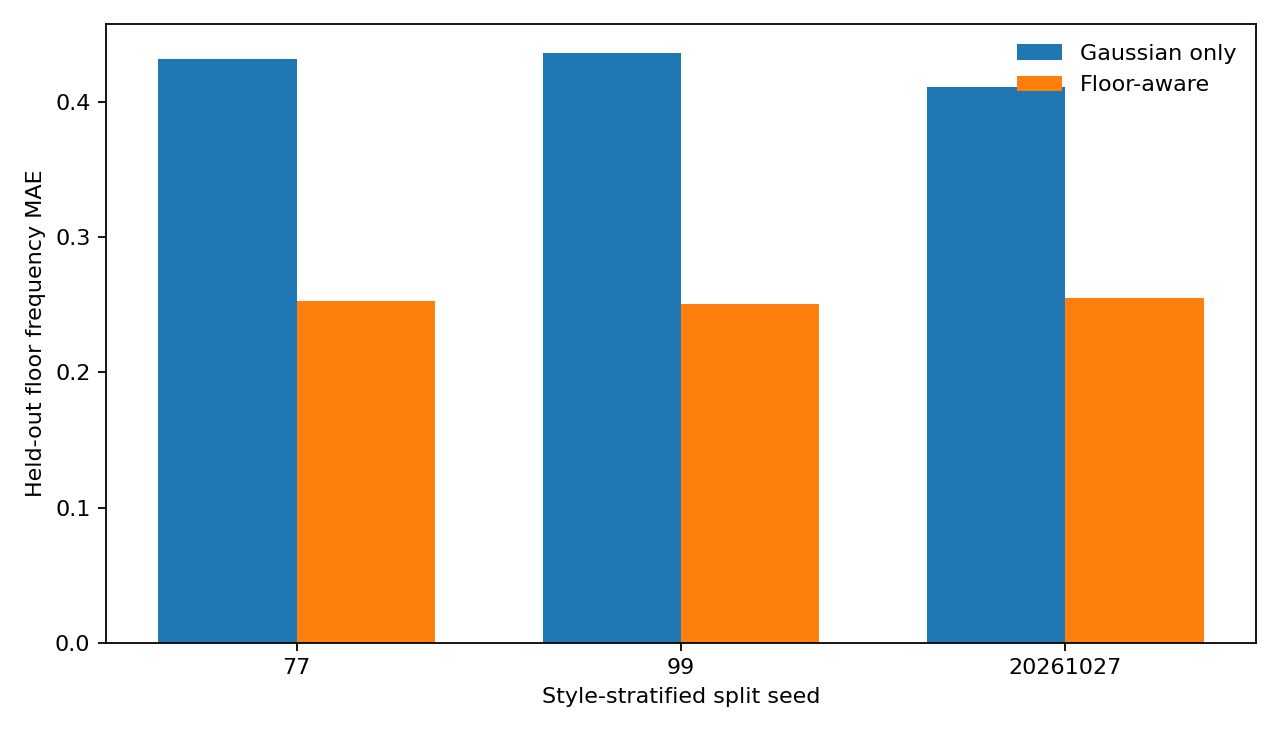
\includegraphics[width=.70\textwidth]{images/figure_floor_calibration.png}
\caption{三次风格分层留出下，最低值质量校准前后的频率误差}\label{fig:floor}
\end{figure}
按风格聚类Bootstrap，绝对MAE改善的95\%区间为$[0.1305,0.2064]$。最终生成22种风格共880条231维谱，使用冻结的第一问ExtraTrees感官代理输出对应50维0--6风味指纹，且父子评分卡约束违反数为零。

\subsection{Bures--Wasserstein传输与逐项缺陷控制}
以Pils/Lager为源、Tripel为目标，在收缩的低维高斯统计量之间使用Bures--Wasserstein最优传输，并通过投影保证DMS、双乙酰、4VG与trans-2-nonenal不超过源化合物的测量值。第五项stale\_hops缺少独立的同名化学浓度，以第一问冻结的感官代理预测分作约束。再从条件Tripel分布采样候选，选取满足约束且对目标潜空间距离较小的谱。
\begin{table}[htbp]\centering\caption{第三问Pils/Lager到Tripel的约束消融（11款源啤酒）}\label{tab:q3ot}
\begin{tabular}{lcccc}\toprule
方法 & 目标距离 & 靠近目标 & 缺陷恶化 & 代理恶化\\\midrule
无约束OT &2.1064&11&33&5\\
四化学约束OT &2.0954&11&0&5\\
五项约束OT &2.5607&7&0&0\\
五项约束+条件优化 &\textbf{1.7716}&7&0&0\\
\bottomrule\end{tabular}\end{table}
\begin{figure}[htbp]\centering
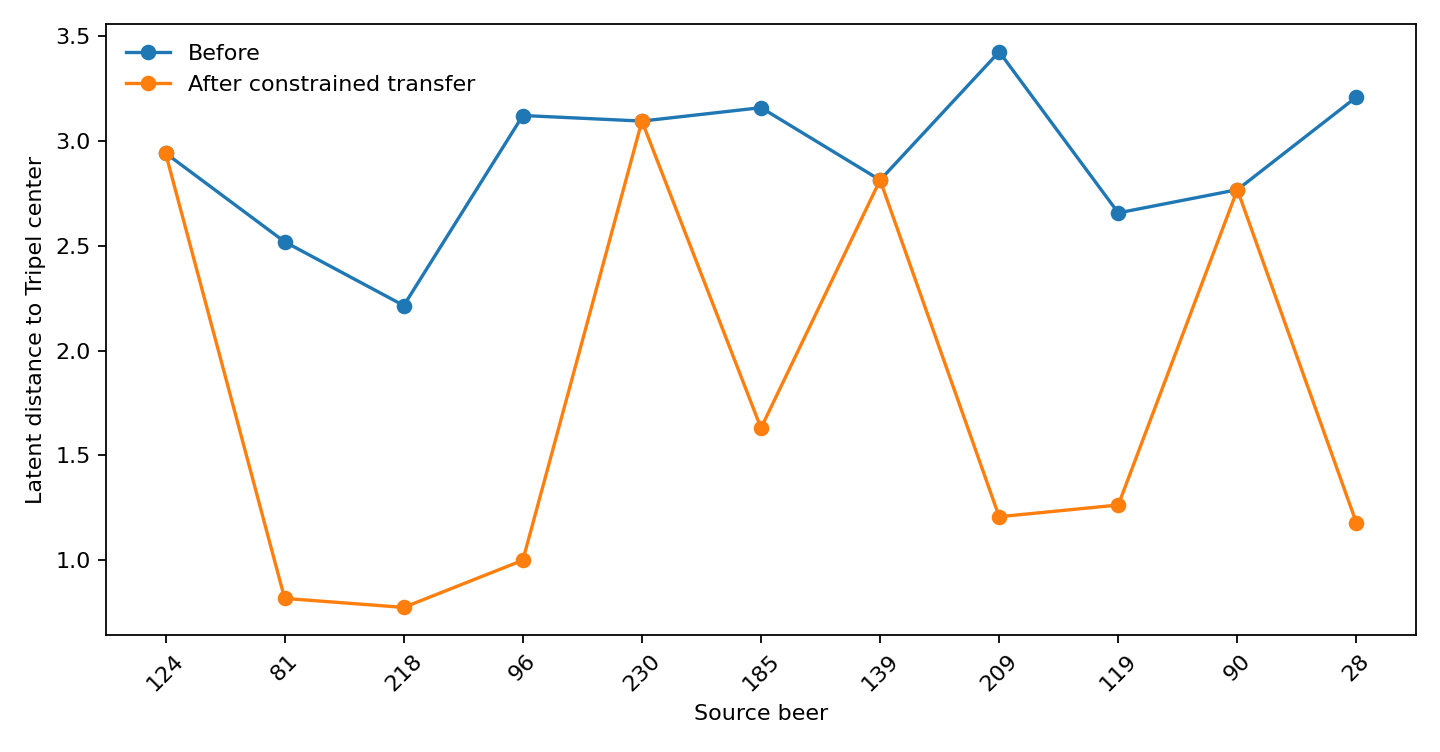
\includegraphics[width=.78\textwidth]{images/figure_transfer_distance.png}
\caption{11款Pils/Lager化合物谱迁移前后至Tripel中心的潜空间距离}\label{fig:transfer}
\end{figure}
源Pils/Lager中有两条双乙酰数值缺失，因此表中实测缺陷比较仅42项；缺失位置采用保守最小值填补，但不能宣称已经核实真实缺陷不恶化。stale\_hops为代理模型预测，不构成真实品评保证。7款靠近目标，另4款保持原谱，不虚报为迁移成功。

\section{检验、限制与结论}
第一问的真实参考均值来自原论文公开数据，覆盖与题目相同的250款啤酒，不构成独立外部数据集。第二问有显著的稀疏预测增益，但选择稳定性仍需提高，化合物关联不代表因果。第三问的最低值分布修正在三套留出样本上均有一致改善，缺陷约束可通过数值消融检验；实验室真实检出限及缺陷感官仍需额外测量。全文报告保留负结果，以可复现建模证据确定最终方案。

\section*{参考文献}
\noindent [1] Schreurs M, et al. Predicting and improving complex beer flavor through machine learning. Nature Communications, 15:2368, 2024.\par\noindent
[2] MathorCup数学应用挑战赛组委会. 2026年MathorCup大数据竞赛赛道A初赛题目，2026.\par\noindent
[3] Schreurs M, et al. Data from: Predicting and improving complex beer flavor through machine learning. Zenodo, doi:10.5281/zenodo.10653704.

\section*{AI工具使用声明（提交前按实际情况修订）}
本稿结构、第一问和第二问研究代码与图表受到OpenAI GPT-6辅助；参赛队须对采用内容的准确性进行独立审查和修改，在正式论文相应位置标注AI辅助贡献，并在支撑材料单独提供\textbf{AI工具使用详情说明（PDF）}，列出模型、时间、使用环节、关键交互与人工修订情况。

\end{document}
